%%%%%%%%%%%%%%%%%%%%%%%%%%%%%%%%%%%%%%%%%%%%%%%%%%%%%%%%%%%%%%%%%%%
%                                                                 %
%                            CHAPTER ONE                          %
%                                                                 %
%%%%%%%%%%%%%%%%%%%%%%%%%%%%%%%%%%%%%%%%%%%%%%%%%%%%%%%%%%%%%%%%%%%

\chapter{INTRODUCTION}

Consider the example... --> Bugzilla.
Requirements for Development of Hypermedia Technology for a Digital Library Supporting Scholarly Work \cite{Wiil:2000:RDH:338407.338517}.
Anyone who has used an iPhone or owned a video game console understands the basics of versioning.
Companies brand sequential devices to indicate that there has been an improvement in performance or capabilities.


%%%%%%  Data changes and grows, we have to track it --> Data Quality?
John C. Maxwell once said, "Change is inevitable.  Growth is optional."
While this inspirational quote refers to the human character, it also holds true for scientific datasets.
With changing technology, data collected by researchers grew at an astounding rate.
NASA's Atmospheric Science Data Center (ASDC) reported a growth from hosting around five million files to twenty million files between 2001 and 2004 as seen in Figure \ref{table:ASDC} \cite{Barkstrom_digitallibrary}.
The ATLAS project at CERN reports that it generates on the order of four thousand new datasets per day from experimental tests alone shown in Table \ref{table:Atlas} \cite{Branco2008}.
The sheer volume of data generated per year by each of these organizations easily demonstrates the futility of managing these data archives manually.
The desire and ease in which data transparency can be provided to not only researchers but also the public lies behind the drive of expanding the availability of high quality data holdings.
The key to meeting these demands is automation, not only in distribution, but also in data quality management.
However, these two dynamics are at odds with each other.
Many NASA datasets have required re-processing of their data, either to improve data quality or to correct for errors \cite{barkstrom2014earth}.
However, we can also see that the number of distinct users doubled over the course of three years at the ASDC while the amount of data distributed more than triples.
As such, the strain of informing and providing updated data to this body of users grows tremendously.
The solution, thus, lies in passing on the ability to verify data quality to the users.
Data traceability now becomes particularly important to identify sources that contribute to improved data quality.
It creates a need to understand not only that a data set has changed, but to also understand how much a data set has changed.
Data versioning is the method of tracking the changes performed on a data set and determining the extent to which it has changed.
In this document, data versioning is approached using technology provided by semantic technologies and applying them to artifacts currently generated by scientific data sets.

\begin{figure}
	\centering
	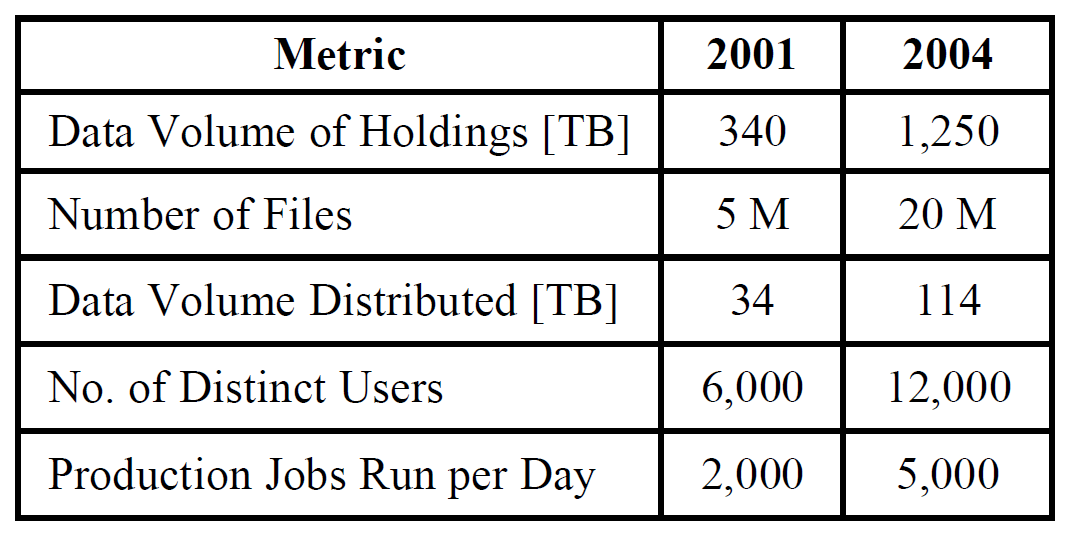
\includegraphics[scale=0.40]{figures/ASDCHoldings.png}
	\caption{Summary of ASDC Holdings for the years 2001 to 2004 from Barkstrom and Bates \cite{Barkstrom_digitallibrary}}
	\label{table:ASDC}
\end{figure}

\begin{table}
	\centering
	\begin{tabular}{ | c | c |}
		\hline
		Metric & Magnitude \\
		\hline
		Data per day [TB] & 1 \\
		Data per year [PB] & 20 \\
		Datasets per acquisition & O(4000) \\
		Simulation Datasets per day & O(1500) \\
		Versions per Dataset & O(1) \\
		Files per Dataset & O(100) \\
		\hline
	\end{tabular}
	\caption{Summary of ATLAS data set generation in 2008 from Branco et al.\cite{Branco2008}}
	\label{table:Atlas}
\end{table}

\section{Defining Versions and Versioning}

Researchers often use the words version and versioning without needing to explicitly defining them because they appear ubiquitously in data management systems.  As a result, the definition of a version varies depending on the application, but they all try to capture a common idea.  Barkstrom describes versions as homogeneous groupings used to control, "production volatility induced by changes in algorithms and coefficients as result of validation and reprocessing," \cite{Barkstrom2003}.  He separates groupings by the granularity at which observations are collected.  This construction allows users to easily determine the similarity or dissimilarity of objects within the grouping.  However, NASA employs a rigid data processing structure with well defined levels.  This means that the resulting hierarchy is well balanced.

Another application defines a version as a "semantically meaningful snapshot of a design object," \cite{Tagger2005}.  

It is more constructive to define versions as a matter of purpose.  When two objects are versions of each other, they are considered to still serve the same purpose.  For data production services, this would translate to there they exist in the workflow. Two objects must, therefore, share provenance, and the more they share, the more likely versioning practices will provide meaningful results.

Versioning is the activity of exposing changes relating two or more versions of an object.  Versioning differs from provenance because an activity does not establish an object as a version of another even though the activity may create it.  The relationships exist as a matter of state-based properties which are exposed through versioning.  These relationships have greater significance if the objects are versions of each other.

\section{Changelogs}

Changelogs, sometimes called patch notes, are artifacts resulting from the versioning process often found in major software projects.
They document the changes made within the system and seek to explain, in human language, the motivations behind changes \cite{uel1037}.
The logs provide significant utility to both users and producers as it can serve as both documentation and tutorials.
Many users will often refer to the patch notes in order to decide how to adapt to changes made to the system they use, either data or software.
Meanwhile, changelogs aid producers through team transitions by keeping a history of decisions made to improve the project.
This is particularly evident in the realm of open-source projects as developers can contribute without having been part of the original development team.
The need for documentation to bring new programmers up to speed for a project drives the ability to keep the project alive.

Open source projects have much more consistent adoption of changelogs than data sets, possibly resulting from complex code techniques emerging earlier than large data methods.
These logs provide a great source of value to developers as they can be used to give insight to the health of a software project \cite{German03automatingthe}.
These projects have a tendency to die rather quickly after initial enthusiasm and with the rather low overhead cost to start new open-source projects, some automated methods of determining the progress of a project is needed.
It would give insight into the maturity of a project's development team as well as the likelihood that team members will correct errors within the code.
However, readability proves to remain a significant hurdle as current development change logs contain solely human readable text.
While machines may still be significantly removed from the ability to comprehend the impact of changes made to a data set or software code, they are currently opaquely blocked from consuming any of the content within logs more than understanding they contain text.
The transition between different versions of large datasets is then left largely up to the human user's ability to understand and process the modifications mentioned within the change log.

As mentioned previously, changelogs also allow developers to link bugs and errors with their corrections in new versions of the code \cite{Chen:2004:OCL:990374.990391}.
This gives feedback to the user community that corrections have been addressed as well as ensuring that modifications to the code base are driven by improving the project.
It also has the added benefit of creating a system that can be used to link the introduction of new features with the emergence of new bugs \cite{6132954}.
The resulting discoveries help reveal patterns of development and prevent further occurrences of problematic code.
Therefore, providing an machine consumable changelog would accelerate and assist in navigating through dataset changes and error corrections.

\subsection{RDFa}

In order address the human readability of data change logs, this project considers the use of the Resource Description Framework in Attributes (RDFa) framework \cite{Adida2015}.
Figure \ref{RDFa} illustrates the semantic difference between what web crawlers and what humans see when they consume web pages.
People intuitively understand that certain strings represent meaningful information, and RDFa seeks to encode that understanding natively into the document in order to allow them the ability to consume the information more effectively.
The framework leverages the existence of various established vocabularies in order to provide a standardized understanding of web documents, and it opens the ability for them to interact with the web pages more intelligently.
The benefits of embedding RDFa into change logs is twofold.
First, the change log would need to be marked up in HTML in order to accept RDFa.
As a result, the log would also become available on-line and thus, more openly accessible to data users through the utilization of web based search engines.
This would allow data users to better determine personally how a change applies to their specific application.
Large companies such as Google have already begun making endeavors in equipping their web crawlers to consume structured data such as RDFa from web pages.
Second, the simple application of RDFa attributes encodes the entries within the change log in a format consumable by machines \cite{Herman2015}.
RDFa has already had significant success in adoption across a variety of web publication platform and eases the search for their content \cite{Bizer2013}.
In these applications, however, the developers use RDFa to describe the content on the page, to indicate a string is actually a name for example.
This project endeavors to use RDFa to embed an RDF graph into the web page instead, and therefore, the data becomes captured instead of described.
The language does have the ability to transform into RDF, but the slight nuance between intended use means that a more complicated deployment of the attributes will be required.
Using a previously established standard eases the adoption of encoding required to communication change information to autonomous systems.

\begin{figure}
	\centering
	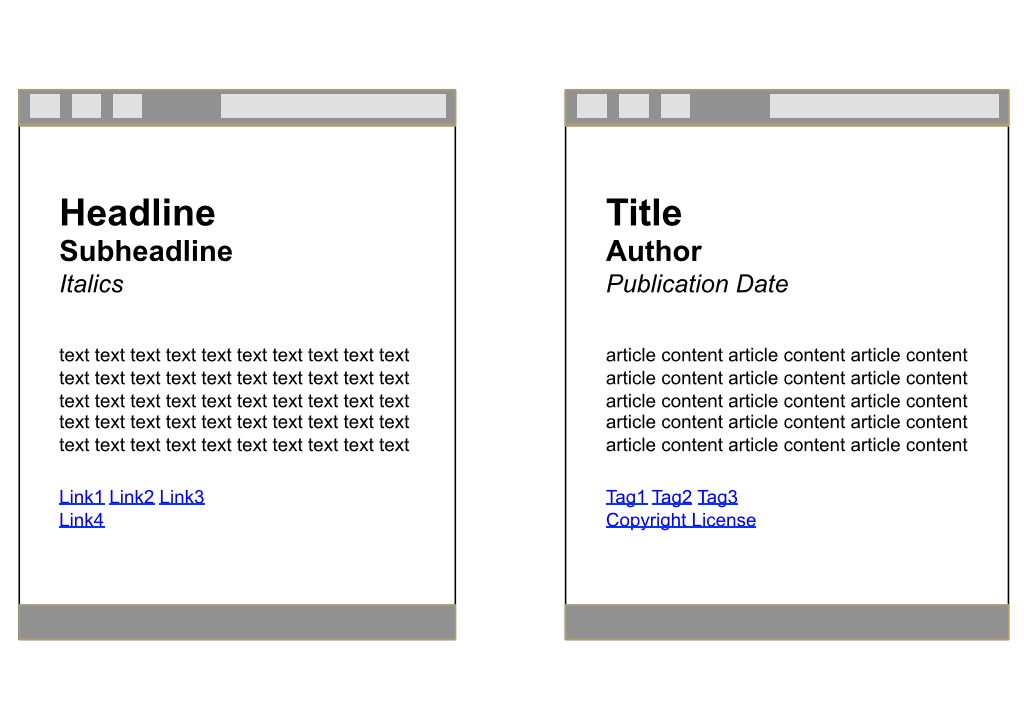
\includegraphics[scale=0.40]{figures/RDFaSemantics.png}
	\caption{Illustration of the difference in what autonomous systems see when crawling a web page and what humans see when reading the same material. Figure 1 from \cite{Herman2015}}
	\label{RDFa}
\end{figure}

\section{Modeling}

It describes the sequence of events that lead to the construction of an object  \cite{dai2014provenance}.

However, a model recently released model by the Health Care and Life Sciences (HCLS) Interest Group may provide a solution when used in conjunction with other identifiers \cite{Dummontier2016}.
Their model, shown in Figure \ref{HCLSModel}, separates the concept of a dataset into three parts.
The highest level summarizes the data as an abstract work, perhaps better described as a topic or title.
This data topic can have multiple versions as it changes over time.
The version can then be instantiated into various distributions with different formats.
Such a set of linked data would provide sufficient data to discern between two data instances of the same information.
However, it is unclear as to whether a single identifier would be able to encompass such complete information.

\begin{figure}%[b]
	\centering
	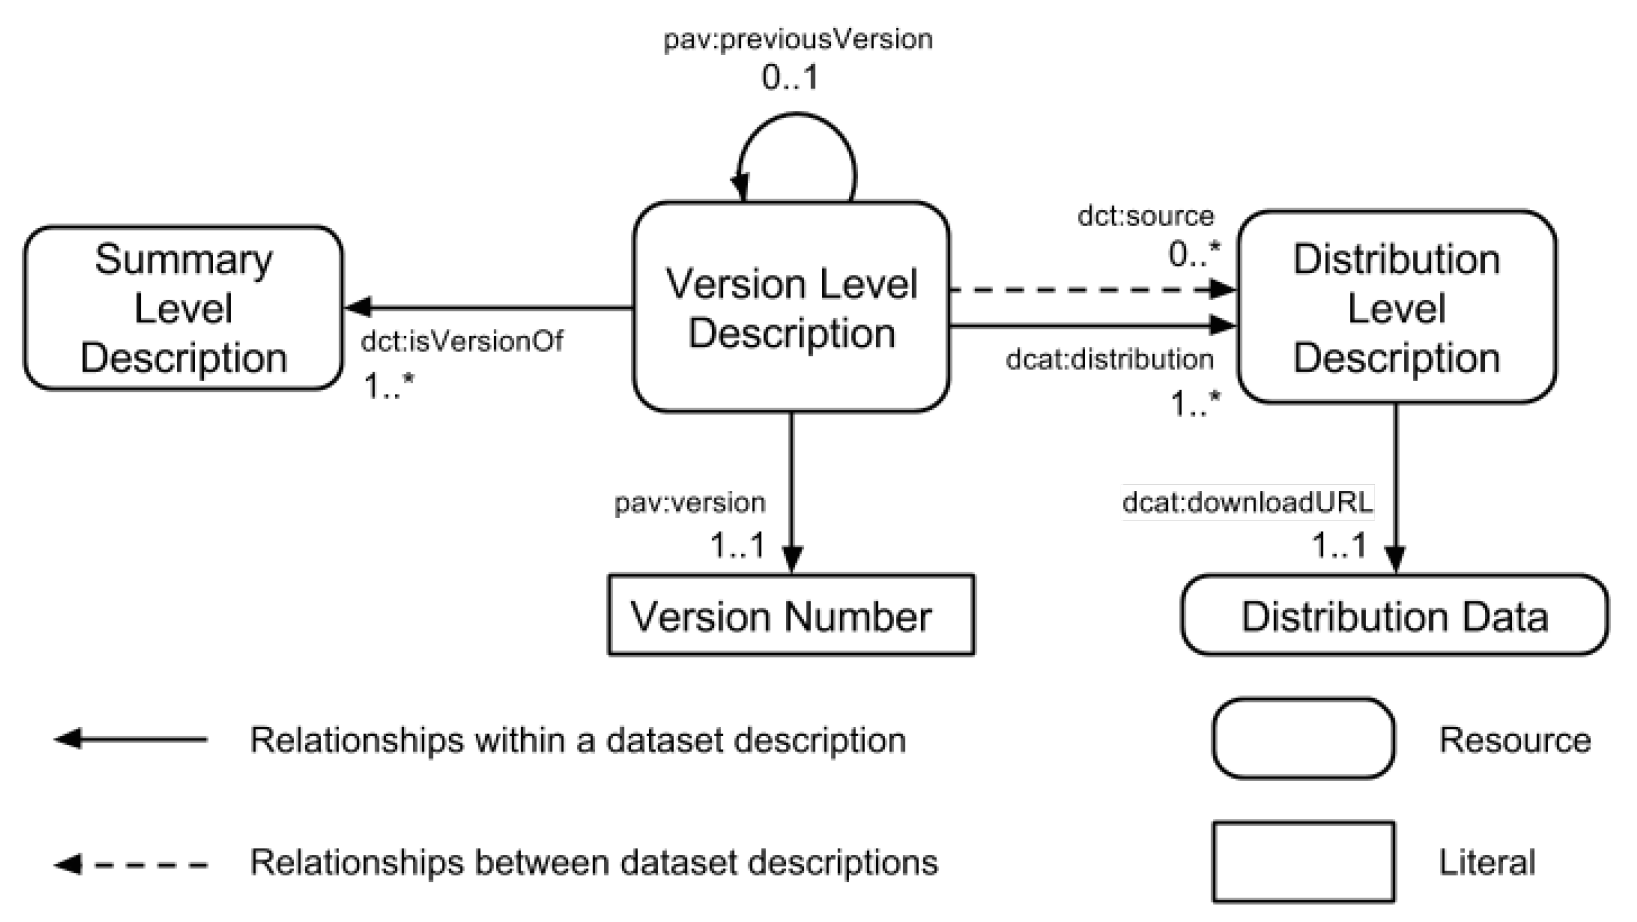
\includegraphics[scale=0.35]{figures/HCLSModel.png}
	\caption{Data model from the Health Care and Life Sciences Interest Group separating data into three levels: works, versions, and instances.  From Dummontier et al. \cite{Dummontier2016}}
	\label{HCLSModel}
\end{figure}

The organization of the model has interesting parallels with Plato's theory of Forms where he proposes that there exists a perfect idea of an object which has imperfect realizations in the physical world.
Likewise, the summary description of the data set represents the ideal which the data seeks to capture.
The model then uses a series of versions represented using the Provenance, Authoring, and Versioning (PAV) ontology to document the physical change of the data as it approaches the ideal\cite{Ciccarese2013}.
PAV produces an interesting entry point into explaining the data set's development as well as recognizing the imperfection inherent in data capture.
As a concept in the model, linked data can further extend the description to provide details necessary in identifying a particular version of data.
However, PAV only has retrospective views of data versions since a version can only point back to previous instances.

\begin{figure}
	\centering
	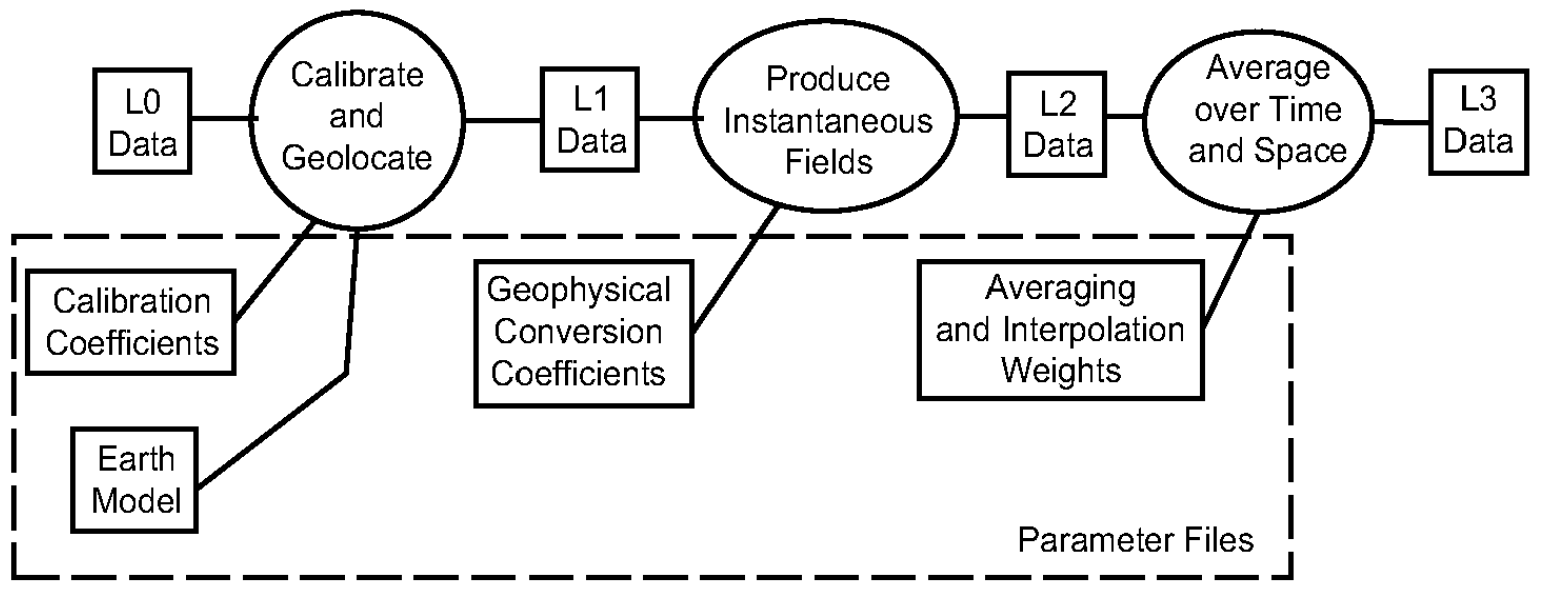
\includegraphics[scale=0.40]{figures/NASALevels.png}
	\caption{NASA organizes its data into three levels depending on the amount of aggregation and the distance the data is removed from the original sensor measurements. Figure 1 from \cite{Barkstrom2003}}
	\label{NASALevels}
\end{figure}

NASA defines three levels of data processing, seen in Figure \ref{NASALevels}, that encompass the stages required to turn a raw signal from satellite instruments into physical measurements into global aggregate summaries \cite{Barkstrom2003}.

\section{Identifiers}

Early citations used stagnant Uniform Resource Locators (URL) to refer to online documents, but this would lead to a condition known as link rot where moving the document would invalidate the URL \cite{Lyons2005}.
This eventually led to the development of Persistent URLs (PURL) which also succumbed to link rot, and this eventually led to the distributed Digital Object Identifier (DOI) system used to track documents today \cite{Duerr2011}.
In the table taken from Duerr et al. \cite{Duerr2011}, DOIs represent the most suitable identifier used for science.
It's origins begin in the Handle system, which can be seen as a generalization of the DOI system.
The DOI network provides a robust system to track documents, but when tracking data, it faces difficulty following the rate of change with some more volatile data sets.
Distribution organizations assign a DOI whenever a new edition of a document becomes available, and due to the publication process, documents change very rarely so a new DOIs are rarely necessary.
However, data sets are products and thus succumb to the iterative process of error correction and growth.
Data collection often continues on after initial publication.
DOI distributors treat new files like new sections to a paper and changes to files as edits so a new identifier must be issued to the data set.
This behavior becomes entirely too slow as data providers begin to allow users to dynamically generate data products from existing data according to their needs \cite{Barkstrom2003a}.

\begin{figure}
	\centering
	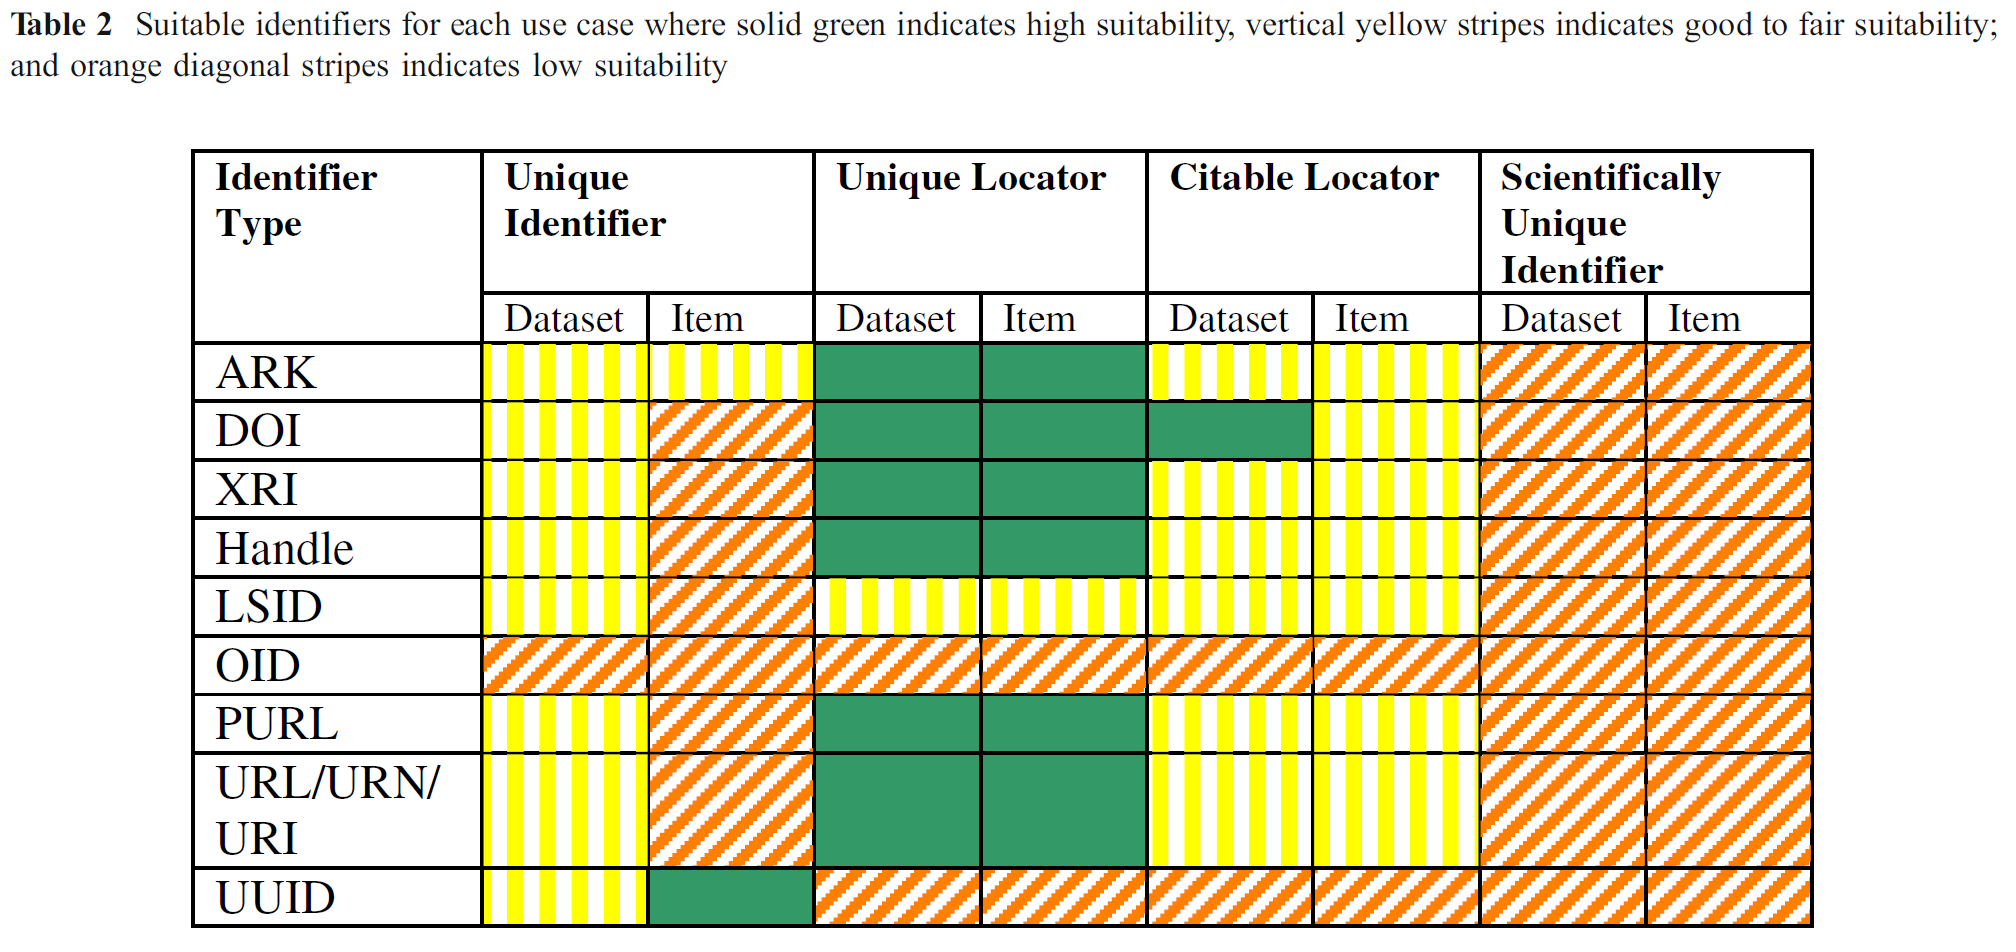
\includegraphics[scale=0.30]{figures/DigitalIdentifierTable.png}
	\caption{Table of predominant identifiers used in science.  From Duerr et al. \cite{Duerr2011}}
	\label{table:Duerr}
\end{figure}

With respect to Figure \ref{table:Duerr}, no identification scheme fits the description of a scientific identifier.
Duerr et al. define a use case to make the argument that scientifically unique identifiers are necessary, ``to be able to tell that two data instances contain the same information even if the formats are different" \cite{Duerr2011}.
This highlights the necessity of being able to discern between the logical content of a dataset and the physical form of that object.
As identifiers often use physical characteristics of the data to make comparisons and determine similarity, a proper representation becomes difficult.

\begin{figure}[b]
	\centering
	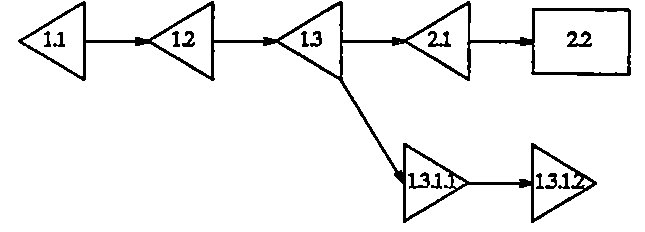
\includegraphics[scale=0.75]{figures/RCSCommitTree.png}
	\caption{Commit history of an object in RCS with changes in the main line stored as back deltas and side branches stored as forward deltas.  Figure 5 in \cite{tichy1985rcs}}
	\label{RCSTree}
\end{figure}

The techniques employed by these technologies, however, can remain applicable to data sets and are often necessary when communicating change data to users.
Version producers often refer to versions using numbers in the dot-decimal style \cite{Stuckenholz:2005:CEV:1039174.1039197}.
While the values often signify the Major-minor numbers associated with the version, the names remain meaningless and can arbitrary assignment such as Ubuntu released numbered by Year-month values \cite{Ubuntu}.
The arbitrary nature of the numbers often entails referring to versions by English nicknames instead.
Such a regular method of naming release versions also means that determining the magnitude of change between two releases becomes impossible.
Numbering the version this way, however, does allow computers and readers to quickly parse the version name and discern that a change has occurred, but little value exists beyond that \cite{Dijkstra1994}.
The technique of distributed and federated employed by GIT does provide significant value to modern methods of versioning data \cite{cederqvist2002version}.
As data workflows and data set dependencies grow, their volatility also expands, meaning that they become more likely to generate new versions.
The federated approach available in the GIT environment allows developers to establish change dams that collect modifications and releasing the data at regular intervals,reducing the changes to a manageable flow.

\section{Data Versioning Operations}

Architecture has a principle that says form follows function, but, for data, form equals function.
As a result, data has as many different forms as it has functions.
Biological experiments often use data within cyclical data workflows where outputs are immediately fed back into new experiments \cite{Tagger2005}.
Even though the goal of the experiment is the final data set, all the intermediary data sets provide significant value in reaching the goal.
Libraries store data about their collections in large databases where both old and new versions of literature need to be maintained \cite{Wiil:2000:RDH:338407.338517}.
Some data exist in such a highly constrained environment that it must be managed at near the hardware level \cite{Flouris04clotho:transparent}.
The struggle no longer becomes generating data, but instead, fitting the data into a format that users find useful and can consume.

The challenge of data versioning systems is to provide a unifying environment that can handle the plethora of forms and functions of its data.
At its core, versioning systems only need to concern themselves with three operations: addition, deletion, and modification.
Most literature surveys do not realize the significance of this commonality as this means that versioning methods can be described by delineating how each operation is approached by a system \cite{Tagger2005} \cite{rohtua}.
Data addition generally constitutes the least complicated versioning operation because it interacts the least with pre-existing data.
However, new data does share context with pre-existing data and provides a method of measuring data set growth.
Since data sets no longer have to be used in its entirety and can be freely subsetted, a data set's complexity increases significantly with its growth.
Every new file added to a data set doubles the number of available subsets.

Data deletion, however, has a more philosophical difference between systems.
From the perspective of a versioning specialist, data should never be deleted since knowing why data was excluded is as important as knowing why data was included.
The software versioning manager GIT uses a method of compressing older data to conserve space without deleting the data \cite{Chacon:2009:PG:1618548}.
Pragmatically, this is not always possible due, generally, to the physical constraints of storage space.
In high energy physics, observational data often cannot be re-collected due to cost, and as a result, poor quality data cannot be re-processed or replaced \cite{Cavanaugh2002}.
The decision in this document is to use the term invalidation when referring to data removal operations as it implies that whether permanently deleted or not, there exists a more valid alternative.

Data modification encompasses the most involved data versioning operation.
As a result, it often comprises a majority of the description of a data versioning service.
In truth, data modification can be summarized as the invalidation of an instance of a data object - which can be a file, a record, or anything in a data set - followed by the addition of a new instance of that data object.
However, this kind of operation is used so often to fix errors and update data sets that it is considered a unique operation.
Modification owes its complexity to interacting with both pre-existing data from the invalidation stage and new data from the addition stage.
However, this compound relationship fully contextualizes the relationship the operation has in relating the old data and the new data.
In some cases, this only provides forward or backwards references between data versions, but having both gives users context for data's current state and update to new data \cite{Klein01ontologyversioning}.

Due to the ubiquity of the data addition, invalidation, and modification operations in versioning systems, the conceptual versioning model presented in Chapter 3 centers around capturing the relationships established by each of the operations.
While other functions exist commonly in versioning systems such as object locking to prevent simultaneous conflicting changes, viewing to see the version an object belongs to, and branching to allow distributed modifications, these functions comprise the space of utility operations that support the three core processes.

\subsection{Types of Change}

The study of versioning operations further breaks down into categorization of change types data sets may undergo.
While the meaning of operations are fairly easy to understand, not all changes have the same impact.
As mentioned previously, version numbering separates perturbations into categories based on the impact the producer believes it has on the project.
In this project, changes are categorized into scientific, technical, and lexical changes.
The granularity of the categorization does not consider the magnitude of change within the individual values stored by a data set as actual values vary depending on application and domain.
Focusing on a more abstract representation of kinds of change allows for a better understanding of its impact while not being too precise to be domain specific.

Scientific changes comprise the family of changes which have the greatest impact on a project or data set.
It indicates that modifications have been made to the most fundamental methods used to create a data set.
These can include changes to algorithms used or sampling methods which may require a change in how users consume the new data.
These changes have the largest implications for data consumers as it can have serious consequences for the soundness of their results.
However, these kinds of changes is not always caught on the production end of data generation.
While very large modifications can easily be determined to produce a scientific change, more subtle changes or interactions can also have larger ramifications, and data producers may initially view this as a technical change due to data quality's subjectivity.
Technical impacts do not change the underlying science of the data, but impose a large enough change as to warrant notice.
Structure alteration and unit conversions count as technical changes since the dataset now needs to be consumed differently but remains valid for use.
In one of the data sets used by this projects, concentration units were originally reported in parts per million and then in cc isotope ratios.
This would constitute a technical change since the data presents the same scientific measurements but in a different manner.
Lexical changes belie the transformations that can best be described as corrections.
Filling in previously missing values or fix erroneous values may be lexical changes.
While they have the smallest impact on results and conclusions, these changes can allow computations to be performed when previously missing data discouraged such behavior.

The exact category that a particular change falls into can be controversial.
The decision to change concentration units from parts per million to milligrams per milliliter poses a Technical change for a data producer.
However, for a data consumer, the change may be viewed as a Scientific change as it invalidates the methods they had previously used.
This conflict in view illustrates the data consumer-producer dynamic.
In general, data producers are in control of the methods of versioning, but data consumers determine the classification of a data change.
Producers tend to use versioning systems to ensure data quality of service through audits and recovery tools \cite{Cavanaugh2002}.
Meanwhile, a consumer will analyze the historical changes and determine the impact this may have to their data use.
As a result, this means that data versioning systems must communicate a dynamic view of the changes in a system contextualized by the user of that data.

\section{Data Set Proliferation}

An interesting statistic to note in Table \ref{table:Atlas} is the order of versions per dataset.
While it does not indicate that the data have marked volatility, it does communicate that the data has a tendency to change over time.
This means that not only does an archive maintain a data set, but it may need to maintain multiple instances of that work over time.
Therefore scientists need the ability to discern between instances of the data they use when comparing results from other researchers.
With the web's development, libraries and library sciences provide a steady evolution in methods to identify data collections.
The challenges and goals that face physical libraries remain valid even as data collection migrates to electronic alternatives \cite{rohtua}.
Digital storage and the Internet has opened new opportunities and methods to administer book data by separating logical representations and physical representations \cite{Barkstrom_digitallibrary}.
Publications, for instance, may be sorted and rearranged in a digital view along a wide array of characteristics to provide the most logical presentation for searching.
Comparatively, users search a physical collection by conforming to a rigid organizational system adapted to the provider's needs, not the user. 
It has also added a plethora of new content types such as wikis, blogs, and other document formats which have never seen physical print.
All these new documents need a form of data management \cite{Berberich:2007:TMT:1277741.1277831}.
However, the migration has not been without its problems.

For similar reasons, treating data as documents produces problems when applying technologies from software management \cite{tichy1985rcs}\cite{Chien:2000:VMX:646544.696357}.
Structure provides the most significant distinguisher between data and software since a data set with a removed file remains usable but a software project would break.
The function of code comes from its content, but the function of data comes from its ability to store and organize data.
This should not be confused with data formats which impose structure onto data in much the same way programming languages provides a medium to express actions.
However, exporting data in different formats is currently easier than exporting code into different languages.
Data sets do not represent a single object, unlike a software project\cite{Chacon:2009:PG:1618548}.
They are compact representations of all possible subsets of the data set, which are also datasets.
The Atmospheric Radiation Measurement (ARM) Program publishes data daily from sensors deployed across the globe, but a user may only desire files from a specific region, files from only the year 2012 in the Southern Great Plains region, or from only the month of February for the collection site's lifespan \cite{6906868}.
These can all be considered arbitrary subsets from the data sets generated by the data collection program, but a software project would not be able to sustain such arbitrary filtering.
GIT stores the files comprising a repository as snapshots of each file in the store, and when developers make changes to a file, the store creates a new snapshot of that files as seen in Figure \ref{GITFile}.
A version then becomes defined by the complete collection of snapshots within the repository at the time, and the files cannot be subsetted due to the dependencies between the files in the version.
As a result, when modeling the commit history, or the history of versions, the set of files can be compacted since all components are necessary to produce the object.
Demonstrated in Figure \ref{GITTree}, a developer creates a branch of the master line with commit C3 from C2.
The entire repository at C2 gets copied into the branch, and when the work is done, it gets merged back into the master branch.
When a user then orders the software generated by this repository, it results from the compilation of the entire commit whereas a data set does not require the same completeness to be used.
For this reason, the structures of data sets and software becomes incompatible and software versioning technologies are insufficient to capture this nuance.

\begin{figure}
	\centering
	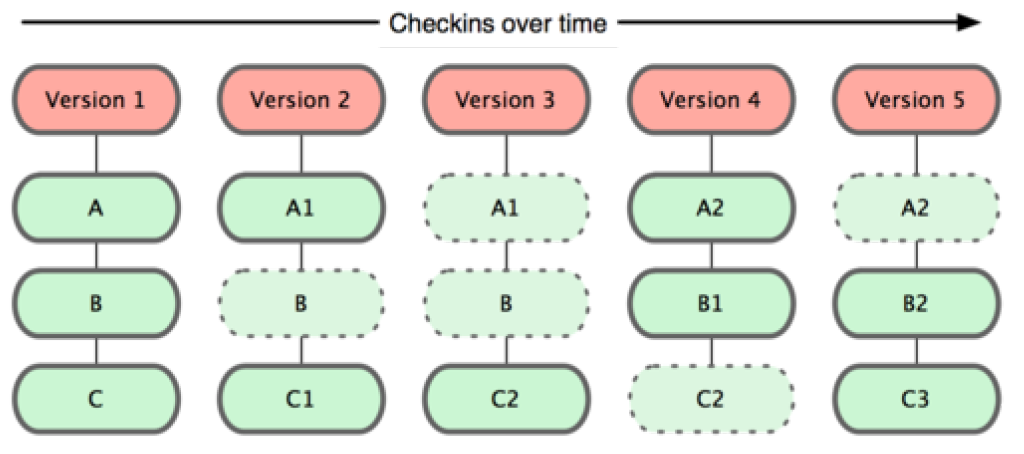
\includegraphics[scale=0.50]{figures/GITFiles.png}
	\caption{GIT stores changes in the repository as snapshots of individual files. Figure 1.5 from \cite{Chacon:2009:PG:1618548}}
	\label{GITFile}
\end{figure}

Furthermore, returning to Figure \ref{GITFile}, GIT actually can be considered a reduction in terms of software versioning methodology.
The constant dynamic in play with tracking versions, perhaps with Computer Science in general, is the trade off between space and time.
Maintaining full snapshots of repositories proves extremely space consuming, but retrieving these snapshots occurs near instantaneously.
In general, prior to this, the conventional wisdom was to instead store one snapshot and a set of deltas or differences between software documents and then use processing time to reconstruct a particular commit by applying the differences \cite{tichy1985rcs}.
Deltas can further break down into forward or backward changes, reflecting the importance of keeping the snapshot of the oldest or newest instance.
This produced very lean versioning systems, but after a long string of changes, applying deltas becomes very time consuming so periodical snapshots become necessary.
With costs for storage space compared to the relative size of software files dropping, GIT prioritizes the ability to quickly swap between and develop different branches of the system.
This interplay between space and computation time can also be seen within the data management space as keeping snapshots of large databases will be intensely costly but less so for spreadsheets.

\begin{figure}
	\centering
	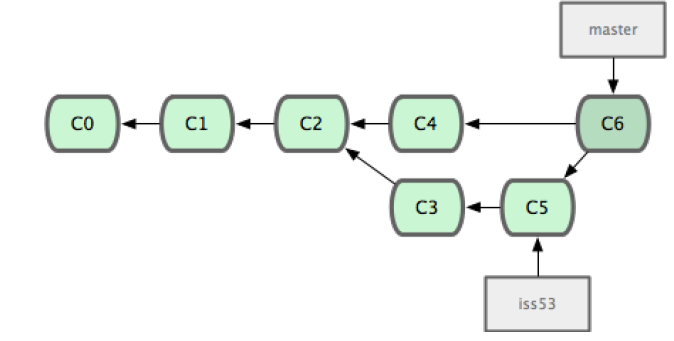
\includegraphics[scale=0.75]{figures/GITCommitTree.png}
	\caption{Example of a commit history with branching stored in GIT.  Figure 3.17 from \cite{Chacon:2009:PG:1618548}}
	\label{GITTree}
\end{figure}

\subsection{Unified Systems}

Working with data as documents leads to the shortfall of technologies, but working with the data of documents has led to significantly greater contributions.
Many libraries often work in collaboration in order to provide a wide selection of texts over a limited number of physically available documents.
The University of Virginia demonstrates the ability to achieve a unified library system using a combination of XML and web service technologies of their disparate assemblage of libraries \cite{Payette2002}.
The challenge involves providing a common landscape in order to compare the quality requirements imposed on the repositories.
Versioning systems provide a notable mechanism to make this decision as quality determines when to generate new versions and what items belong to the same groupings of data.
The comprehensiveness of XML and web technologies also allows this approach to apply to other systems and research areas as well.
This becomes particularly relevant as innovations in computation technology generates small, volatile data sets to integrate into larger data managers \cite{Baker2009}.
In this application, the data food chain then becomes represented by smaller applications generated in situ and then unified with other data sets as they move up the food chain to a large, unified data distribution center.

Unified libraries represent a part of a larger collection of systems that rely on the propagation of data through heterogeneous systems to produce rapid complex solutions.
The grid provided a unique environment that had to handle a variety of inputs, and therefore, different input data could run on distinct sets of grid services.
This meant that different versions of the same data could be generated by differing services on the same grid \cite{Kovse2003VGridAVS}.
The CERN grid for the Compact Muon Solenoid experiment separates the physical and logical storage of files, allowing multiple users to refer to the same file without needing to copy the file across the grid \cite{Holtman:687353}.
While the structure and construction of the grid reduced the uncertainty introduced by varying hardware, it raised questions on data quality by abstracting the transparency to underlying services.
Cloud services have recently replaced the grid due to its flexibility in the services available to its autonomous systems.
As the scale and complexity of autonomous systems grow, it becomes more difficult for one system or organization to manage all the circles necessary to produce data deliverables.
The ability to propagate relevant data change data across autonomous systems then assures valid quality in interactions between domains \cite{Systems02champagne:data}.
Not only does this ensure uniformity through system interaction, but it also ensures transparency with respect to the data and methods used to produce conclusions \cite{Tagger2005}.
This often means that systems will need to negotiate a contract and establish a mutual interface to exchange data.
Occasionally, this contract can be formal, but more ideally, the establishment of a standard lineage model or format would allow a greater variety of systems to interact with each other without needing lengthy contractual exchanges.

\section{Data Quality/Provenance}

The fundamental challenge to determining data quality, its subjectivity, needs clarification.
Conceptually, a data set on desert climate likely has very poor data quality and relevancy to a study in whale biology.
However, in a more quantitative sense, that same desert climate data can have excellent quality with respect to its correctness, expression, and traceability.
With the hybridization of data sets from disparate agencies to provide big data solutions, collaborations plays an ever present role in achieving broad, valid findings.
This requires good quality data and the ability to determine when data with better quality becomes available.
The primary focus, generally, involves tracing the lineage of artifacts and activities that lead to the current data.
This provides insight into possible sources of error as well as validating the assumptions made in generating a data set for future use.

There are several characteristics that can describe a data's quality, but the one most relevant to data versioning is provenance.
In art this describes the sequence of people who have had ownership of a piece of artwork.
For data, provenance relates the history of inputs and operations that result in a data object such as a plot or data set.

Each stage computes a dataset using a collection of input data, processing scripts, and calibration values.
This collection forms the provenance for the resulting level of data, and it contributes to the production history of the higher level products it feeds into.
More specifically, scripts and code which "Produce Instantaneous Fields" operates on "L1 Data" using "Geophysical Conversion Coefficients."
The diagram clearly illustrates that should "Calibration Coefficients" used to generate "L1 Data" change, the resulting data would cause "Produce Instantaneous Fields" to yield different "L2 Data."
As such, strong ties lie between identifying versions and locating differences between provenance changes.

As data sets grow, this process becomes even more confusing to coordinate so version control systems often manage provenance.
Current research endeavors to provide high quality data clearly becomes more formalized as data becomes concentrated in massive data warehouses \cite{Vassiliadis1999}.
The focus of a majority of versioning research focuses on lineage retrieval which becomes ever important as evidence grows that researchers generate data faster than they can reasonably track \cite{Bose:2005:LRS:1057977.1057978}.
This poses a particularly difficult problem as provenance provides a potent means of data auditing.
With provenance, data producers ensure the trustability of their data inputs, either ingested from external sources or integrated from internal data sets.
Fairly reassuring results have been found when combining lineage management and error reporting systems \cite{Fischer2003}.
The errors provide a context for the changes made to advance the lineage of the data set and the version manager demonstrates that a problem has been addressed and how it was corrected.
This system becomes extremely important when considering that agency funding often depends on the ability to account for the value of a project's dataset \cite{Cavanaugh2002}.
The data analytics required to determine the value of data collected by a project also requires the provenance to ensure that the analysis is also reproducible.
The basic provenance often collected by hand now needs to be collected automatically in order to facilitate collaboration, especially with projects that are farther away from the data.

\section{Thesis Statement}

The growth of innovative data capturing and storage technologies has led to new challenges in properly tracking the changes stored data sets undergo.
Researchers store data in a variety of formats, from documents to databases, but since the growth in project scope, many have relied on versioning methods from software management technologies to track their data's evolution.
However, these techniques fail to properly capture the changes data undergoes because they do not take into account the impact that a data's structure has on its function.
In order to maintain data quality, producers use provenance meta-data capture the series of activities and agents involved in generating a data entity.
Emergent technologies and frameworks have been developed to digitally capture this information including OPM and PROV.
This data can be used to give insight into the magnitude of change a data entity has undergone by comparing the differences in provenance between the two entities, but this can only be done in broad strokes without more detailed change data.

By looking at the versioning transactions operating on a data set, data consumers can have a better idea as to the extent their data changes.
This thesis document develops a concept model to formally characterize the activities and relationships among data objects when transitioning between versions.
The model would improve current discussion on data versioning by providing a common understanding of terms and activities, changing versioning from a rule of thumb chore to a valuable research activity.
It then demonstrates the model's utility by applying it to tabular spreadsheets, and then generalizes it to other contexts.
In addition, this contribution addresses in more detail the problem of measuring change distance, which using only provenance data could not accomplish, by utilizing the graph structure of linked data.
Through this process, it creates and makes accessible machine readable change logs which allows for clearer deductions when comparing the extent of changes.
This enriches the version documentation process without developing new artifacts, but now allows for the introduction of automation into part of the data auditing workflow.
In addition, the method reinforces the need for dynamic, publicly available change information as data becomes more flexible to accommodate research in more diverse fields.


%%% Local Variables:
%%% mode: latex
%%% TeX-master: t
%%% End:
